\section{Estado del Arte}
\subsection{Antecedentes}
El desarrollo de este proyecto se enmarca en un contexto en el que la cantidad de contenidos multimedia ha crecido exponencialmente, especialmente en plataformas digitales como redes sociales, bancos de imágenes o repositorios científicos. Esta disponibilidad masiva de imágenes ha motivado la creación de sistemas de recuperación visual que ayuden al usuario a encontrar contenido relevante de forma rápida y precisa.

Además, la evolución del aprendizaje automático ha permitido aplicar técnicas de análisis visual más avanzadas, así como métodos para procesar lenguaje natural y generar contenido de manera automática. Esta evolución tecnológica sienta las bases del enfoque adoptado en el presente trabajo.

A partir de estos antecedentes, se presenta a continuación una revisión detallada de las principales líneas de investigación actuales relacionadas con la recuperación visual basada en contenido, el procesamiento de lenguaje natural y los modelos generativos condicionados por texto.

\subsection{Sistemas de Recuperación de Imágenes por Rasgos Visuales (CBIR)}
La recuperación de imágenes basada en contenido es un campo de la recuperación de información enfocado en la recuperación de imágenes basada en las características visuales de estas. En CBIR, el usuario selecciona una imagen de referencia y obtiene como resultado las imágenes de una base de datos de datos similares a la introducida.

\subsubsection{Definición}
Los sistemas CBIR determinan las imágenes más similares analizando el contenido visual de la imagen de referencia y comparándolo con las imágenes almacenadas en la base de datos. Específicamente, CBIR evalúa características visuales como formas, colores, texturas e información espacial para calcular la similitud entre la imagen de consulta y las imágenes de la base de datos en función de estas propiedades \cite{baeldung-cbir}.

\subsubsection{Características}
En los sistemas de Recuperación de Imágenes Basadas en Contenido (CBIR), las características visuales desempeñan un papel fundamental en la representación y comparación de las imágenes. Estas pueden ser clasificadas en dos categorías principales:
\begin{itemize}
    \item \textbf{Características globales}: Estas describen la imagen en su totalidad, proporcionando información sobre elementos que abarcan toda la imagen, como la distribución general de colores, la forma global y la textura general.
    \item \textbf{Características locales}:  En contraste, las características locales describen patrones o estructuras específicas dentro de la imagen. Se centran en áreas más pequeñas de la imagen y pueden incluir detalles como puntos de interés, bordes, texturas locales y puntos clave.
\end{itemize}

La combinación de características globales y locales permite una representación más completa y detallada de la imagen, lo que facilita la comparación y recuperación de imágenes basada en sus atributos visuales.

\subsubsection{Medidas de similitud}
Una vez que se han extraído las características de las imágenes, es necesario evaluar la similitud entre las imágenes de consulta y las imágenes almacenadas en la base de datos. Para lograr esto, se utilizan medidas de similitud, que se pueden dividir en dos tipos:
\begin{itemize}
    \item \textbf{Distancia}. 
    \begin{itemize}
        \item Las medidas de distancia cuantifican la diferencia o disimilitud entre dos vectores de características. La distancia se calcula como la magnitud del desplazamiento necesario para ir desde un punto hasta otro en un espacio métrico. En el contexto de CBIR, las imágenes más similares a la imagen de consulta son aquellas cuya distancia a la imagen de consulta es más pequeña.
        \item Algunas medidas de distancia comunes incluyen la distancia euclidiana, la distancia de Mahalanobis y la distancia de Manhattan. Estas medidas se utilizan para calcular la diferencia entre los valores de características de dos imágenes y determinar su grado de similitud.
    \end{itemize}
    \item \textbf{Métricas de similitud}.
    \begin{itemize}
        \item Las métricas de similitud, por otro lado, cuantifican la similitud entre dos vectores de características. Estas métricas miden la similitud angular o la correlación entre los vectores de características y proporcionan una medida de la proximidad entre las imágenes.
        \item Una métrica de similitud común es la similitud del coseno, que mide el coseno del ángulo entre dos vectores de características. Cuanto más cercano sea el valor del coseno a 1, mayor será la similitud entre las imágenes.
    \end{itemize}
\end{itemize}

\subsubsection{Aplicaciones}
El sistema de Recuperación de Imágenes Basada en Contenido ofrece una variedad de aplicaciones en distintos sectores. En la industria de la moda, optimiza la búsqueda de productos, permitiendo a los usuarios encontrar prendas y accesorios similares a partir de una imagen, lo que mejora la experiencia de compra en línea y la recomendación de productos. Además, en seguridad y vigilancia, el CBIR facilita la re-identificación de individuos en diferentes escenarios, utilizando características visuales como la ropa y el peinado para rastrear a personas específicas.

Por otro lado, en el ámbito del comercio electrónico, mejora la navegación y selección de productos al permitir a los usuarios descubrir artículos similares basados en una imagen de referencia, aumentando así la satisfacción del cliente y las ventas en línea. Asimismo, en aplicaciones de teledetección y análisis geoespacial, el CBIR es útil para el análisis de imágenes satelitales, ayudando en la identificación y clasificación de características terrestres y cambios ambientales. \cite{li2021recent}

Estos ejemplos de aplicaciones exponen la versatilidad del Sistema de Recuperación de Imágenes Basada en Contenido. Su capacidad para mejorar la experiencia del usuario, optimizar la búsqueda de productos y facilitar análisis detallados en teledetección resalta su importancia en la transformación digital actual.

\subsubsection{Diferencias entre TBIR y CBIR}
La siguiente tabla presenta una comparativa entre el enfoque estudiado (CBIR) y la recuperación de imágenes basada en texto (TBIR). Cada enfoque tiene sus propias características distintivas que afectan su eficacia, fiabilidad y escalabilidad. Esta comparativa busca ofrecer una visión general de las fortalezas y debilidades de cada enfoque, ayudando a entender mejor sus aplicaciones y limitaciones.

\begin{table}[H]
    \centering
    \renewcommand{\arraystretch}{1.5}
    \begin{tabular}{p{5cm}p{5cm}p{5cm}}
        \rowcolor{gray!30}
        \textbf{Característica} & \textbf{TBIR} & \textbf{CBIR} \\
        \rowcolor{gray!10}
        \textbf{Método de búsqueda} & Utiliza palabras clave, anotaciones o descripciones textuales & Analiza características visuales como formas, colores, texturas e información espacial \\
        \addlinespace
        \textbf{Proceso de anotación} & Anotación manual por expertos & No requiere anotación manual, analiza el contenido visual directamente \\
        \rowcolor{gray!10}
        \textbf{Dependencia humana} & Alta dependencia de percepciones e interpretaciones humanas & Menos dependencia de la interpretación humana, más objetivo \\
        \addlinespace
        \textbf{Fiabilidad de etiquetas} & Puede ser menos fiable debido a variaciones en la interpretación humana & Mayor fiabilidad al comparar características visuales objetivas \\
        \rowcolor{gray!10}
        \textbf{Eficiencia} & Menos eficiente debido al tiempo requerido para la anotación manual & Más eficiente al analizar directamente el contenido visual \\
        \addlinespace
        \textbf{Escalabilidad} & Puede ser menos escalable debido al trabajo manual requerido & Más escalable ya que no depende de la anotación manual \\
        \rowcolor{gray!10}
        \textbf{Precisión en la recuperación} & Varía según la precisión de las anotaciones y etiquetas & Alta precisión al basarse en características visuales \\
    \end{tabular}
    \caption{Comparativa TBIR vs CBIR}
    \label{tab:tbir-cbir}
\end{table}


\subsection{Redes Neuronales}
En el ámbito de la inteligencia artificial y el aprendizaje automático, las redes neuronales han surgido como una potente herramienta para modelar y analizar datos complejos. Representan una vanguardia en estos campos, impulsando innovaciones tecnológicas y transformando la manera en que interactuamos con la información y el mundo que nos rodea.

\subsubsection{Fundamentos}
Las redes neuronales se basan en la simulación de la estructura y el funcionamiento del cerebro humano para procesar información \cite{redes-open}. Están compuestas por un conjunto de nodos conectados entre sí que reciben y procesan información y generan una salida en consecuencia. Estos nodos, llamados neuronas artificiales, pueden ser ajustados para mejorar la precisión de la salida, permitiendo así un aprendizaje y adaptación de la red.

La estructura de una red neuronal se compone de múltiples capas de neuronas interconectadas entre sí. Estas capas incluyen una capa de entrada, que recibe los datos iniciales y los introduce en la red, y una capa de salida, que produce el resultado final o la predicción deseada. Además, entre la capa de entrada y la capa de salida, puede haber una serie de capas ocultas que desempeñan un papel crucial en el procesamiento y la transformación de la información a medida que se propaga a través de la red.

\begin{figure}[H]
    \centering
    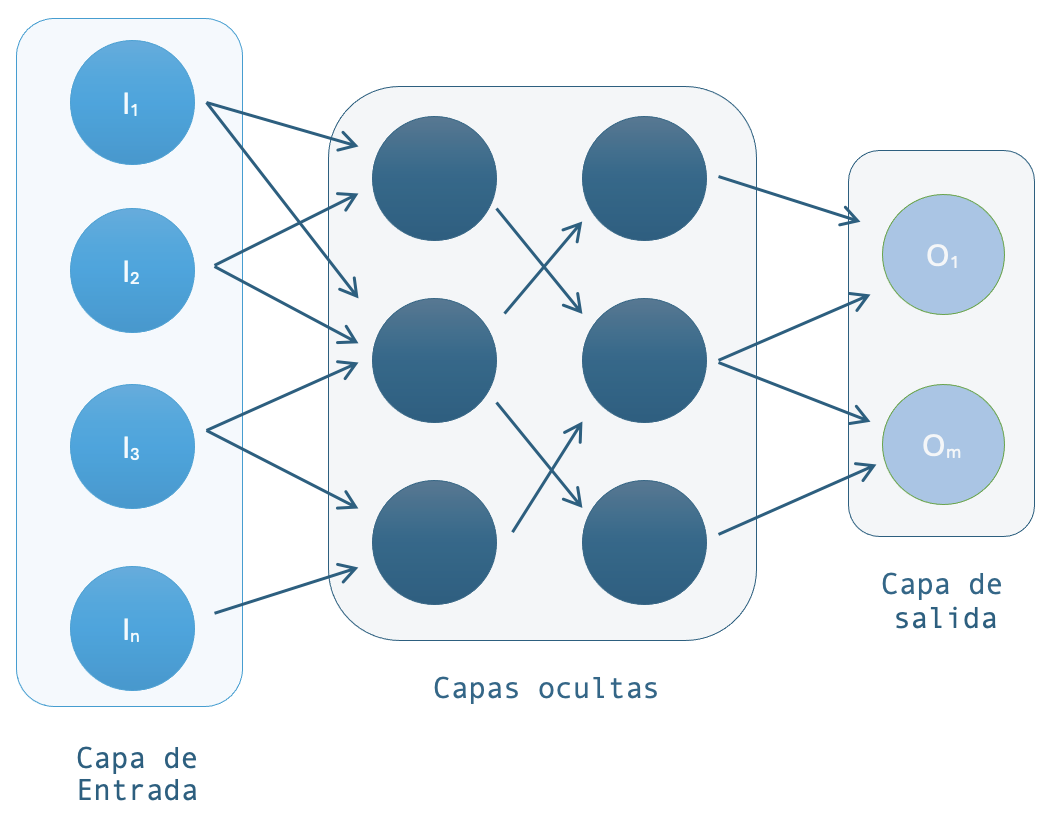
\includegraphics[width=0.6\textwidth]{red-neuronal.png}
    \caption{Estructura de una red neuronal}
    \label{fig:red-neuronal}
\end{figure}

Cada neurona en la red está conectada con otras neuronas mediante conexiones, similares a las sinapsis en el sistema nervioso biológico. Estas conexiones determinan la fuerza y la influencia de la información transmitida entre las neuronas. Durante el proceso de entrenamiento de la red neuronal, estos pesos sinápticos se ajustan y optimizan continuamente a través de algoritmos de aprendizaje con el objetivo de mejorar la precisión y la eficiencia de la red en la tarea específica para la que ha sido diseñada.

El proceso de entrenamiento es un ciclo iterativo que implica alimentar la red con datos de entrada y comparar la salida producida con la salida esperada. Si existiese una discrepancia entre estas, se realizarían ajustes en los pesos de las conexiones.

\subsubsection{Funciones de activación}
Las funciones de activación son una parte crucial del funcionamiento y la capacidad de aprendizaje de las redes neuronales. Estas funciones determinan la salida de cada neurona en función de la entrada que recibe, proporcionando una forma de introducir no linealidad en el modelo y permitir a la red aprender y modelar realciones complejas en los datos.

Existen dos tipos principales de funciones de activación: lineales y no lineales. Las funciones lineales son más simples y se limitan a multiplicar la entrada por un peso y sumar un término de sesgo, lo que resulta en una transformación lineal de los datos. Por otro lado, las funciones no lineales introducen la no linealidad, permitiendo a la red capturar y representar relaciones más complejas entre las variables de entrada y salida.

Algunas de las funciones de activación más comunes utilizadas en las redes neuronales son Sigmoide, ReLu y Tanh.

\begin{itemize}
    \item La \textbf{función Sigmoide} tiene una forma característica de ``S'' y se define matemáticamente como \begin{equation}
        f(x) = \frac{1}{1 + exp(-x)}
    \end{equation} Esta función produce una salida en el rango de 0 a 1, lo que la hace especialmente útil en problemas de clasificación binaria donde se busca predecir una probabilidad entre dos clases.
    \item La \textbf{función ReLu} es una de las funciones de activación más populares en las redes neuronales modernas. Se define como \begin{equation}
        f(x) = max(0, x)
    \end{equation} lo que significa que la función retorna cero para valores negativos y la misma entrada para valores positivos.
    \item La \textbf{función Tanh} es similar a la Sigmoide, pero produce una salida en el rango de -1 a 1. Matemáticamente se define como \begin{equation}
        f(x) = \frac{exp(x) - exp(-x)}{exp(x) + exp(-x)}
    \end{equation} Esta función es útil en problemas de clasificación binaria y regresión donde las salidas pueden ser negativas.
\end{itemize}

\subsubsection{Tipos}
Cada red neuronal está diseñada para atender requisitos diferentes en el proceso de datos según las necesidades del usuarios. Las más prominentes en aplicaciones actuales son las redes feedforward, recurrentes y convolucionales. 

\begin{itemize}
    \item Las \textbf{redes feedforward} representan el modelo más básico de red neuronal. En este tipo de arquitectura, la información se mueve en una dirección única, desde la entrada hasta la salida, sin la presencia de ciclos o conexiones retroalimentadas. Cada capa procesa la información y la transmite a la siguiente capa, siguiendo este flujo unidireccional hasta obtener la salida final.
    Este diseño de red es epecialmente adecuado para aplicaciones de clasificación y predicción, como el reconocimiento de imágenes o la detección de actividades fraudulentas.
    \item Las \textbf{redes neuronales recurrentes} (RNN) se caracterizan por tener conexiones que retroalimentan las neuronas entre sí. Esta estructura permite que la salida de una neurona sea utilizada como entrada para otra, creando así una ``memoria'' que conserva información sobre los datos de entrada previos. 
    Debido a su capacidad de retención de información, las RNN son especialmente efectivas en tareas que implican el procesamiento de secuencias, como el análisis de lenguaje natural y la predicción meteorológica.

    \item Las \textbf{redes convolucionales} (CNN) fueron específicamente diseñadas para el procesamiento de imágenes y vídeos. En estas redes, las neuronas se agrupan en capas convolucionales, donde cada neurona se conecta únicamente con una región local de la capa anterior mediante una operación de convolución, definida por \begin{equation}
            S(i, j) = (K \ast I)(i, j) = \sum_{m}\sum_{n} I(m, n) \cdot K(i - m, j - n)
    \end{equation} Esta organización permite que la CNN identifique características particulares en una imagen, como contornos y texturas, sin importar su ubicación dentro de la misma.
\end{itemize}

\subsubsection{Aplicaciones}
En la actualidad, las redes neuronales desempeñan un papel fundamental en la transformación de diversos campos tecnológicos, y su aplicación se extiende a una gran variedad de industrias y áreas de investigación. A medida que esta tecnología avanza, se desarrollan nuevas aplicaciones que aprovechan sus capacidades de aprendizaje y adaptabilidad para resolver problemas complejos y mejorar la eficiencia en diferentes sectores.

Por ejemplo, el transformador de lenguaje basado en redes neuronales GPT-4 ha marcado un hito significativo en el campo del procesamiento del lenguaje natural. Este modelo es utilizado en diversas plataformas y sevicios, como ChatGPT, un asistente virtual para la interacción con los humanos; DALL-E, que genera imágenes únicas a partir de descripciones textuales; y Riffussion, una herramienta para la composición musical y la creación de melodías basadas en texto.

\begin{figure}[H]
    \centering
    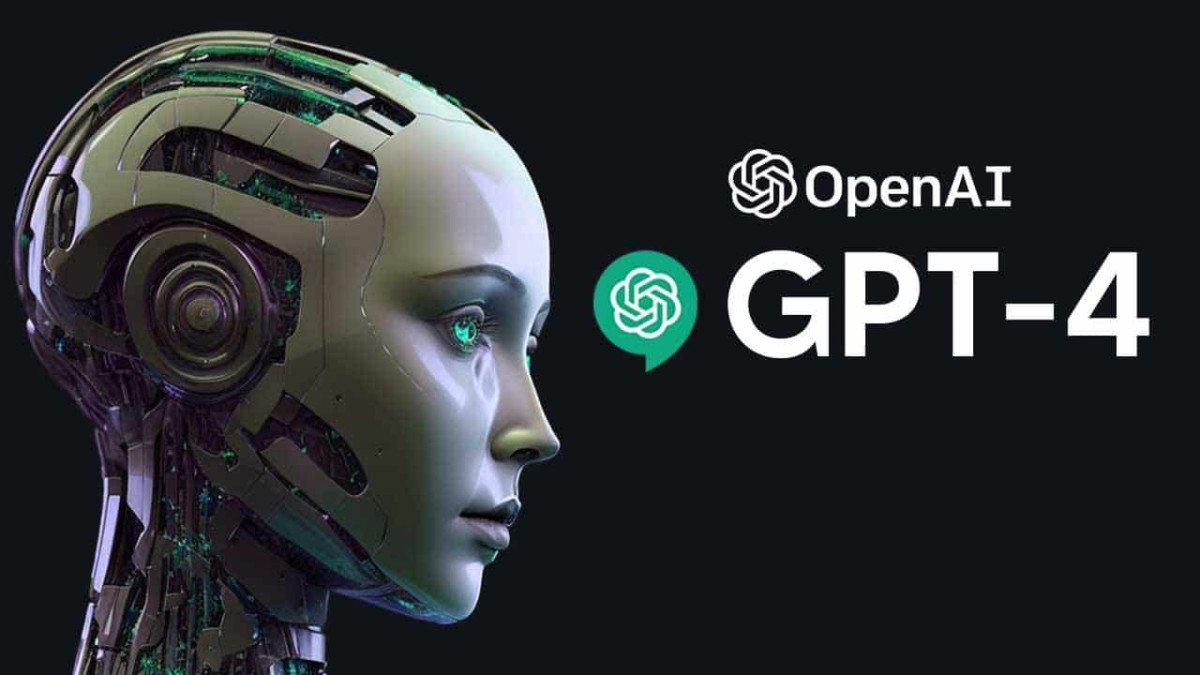
\includegraphics[width=0.5\textwidth]{GPT-4.jpg}
    \caption{GPT-4}
    \label{fig:GPT-4}
\end{figure}

Estos ejemplos muestran la versatilidad de las redes neuronales en la actualidad, demostrando su potencial para impulsar la innovación en múltiples ámbitos.

\subsection{Redes Generativas Adversarias (GAN)}\label{subsec:gan}
Las Redes Generativas Antagónicas (GAN) son una arquitectura especializada de redes neuronales profundas que consta de dos componentes principales: el generador y el discriminador. Estas redes operan en un ciclo de retroalimentación constante, compitiendo entre sí en un proceso antagónico para generar datos sintéticos de alta calidad que sean indistinguibles de los datos reales. Este carácter antagónico y su capacidad para generar datos sintéticos versátiles hacen que las GAN sean una herramienta poderosa con aplicaciones innovadoras en diversos campos del aprendizaje automático y la inteligencia artificial. \cite{gan-mathworks}

\subsubsection{Componentes}
Las GAN se distinguen por su arquitectura única, compuesta por dos elementos que trabajan en sinergia: el generador y el discriminador. Mientras que el generador se encarga de producir instancias de datos que imitan a los datos reales, el discriminador actúa como un crítico, evaluando y diferenciando entre los datos generados y los datos reales. Esta dinámica antagónica entre el generador y el discriminador impulsa la mejora continua y la generación de datos sintéticos cada vez más realistas.

\begin{enumerate}
    \item \textbf{Generador:}
    \begin{itemize}
        \item El generador, concebido como un ``artista digital'', opera en un espacio de alta dimensionalidad utilizando un conjunto inicial de números aleatorios (ruido). Este proceso puede ser visualizado como la falsificación de una obra de arte en un lienzo en blanco, donde el generador transforma hábilmente este ruido en datos representativos de la distribución de los datos reales.
        \item  La esencia del generador reside en su capacidad para generar datos que, al ser evaluados, resulten indistinguibles de los datos reales. Este desafío intrínseco impulsa al generador a capturar de manera fiel las características inherentes al conjunto de datos de referencia.
    \end{itemize}
    
    \item \textbf{Discriminador:} 
    \begin{itemize}
        \item El discriminador desempeña el papel de un crítico discerniente. Su tarea consiste en evaluar los datos presentados y distinguir de manera aguda entre los auténticos y aquellos generador por el modelo. Su evolución se centra en la mejora constante de esta capacidad discriminatoria.
        \item La meta primordial del discriminador es perfeccionar su capacidad de discernimiento entre datos reales y generados. Su agudeza se traduce en un desafío constante para el generador, estimulando un proceso de mejora continua.
    \end{itemize}
\end{enumerate}

\subsubsection{Proceso de entrenamiento}
El entrenamiento de las Redes Generativas Adversarias permite a la red aprender y perfeccionar su capacidad para generar datos sintéticos de alta calidad. En este proceso, el generador busca generar datos sintéticos que sean cada vez más indistinguibles de los datos reales, mientras que el discriminador se esfuerza por mejorar su capacidad para distinguir entre datos generados y datos reales.

\begin{enumerate}
    \item \textbf{Inicialización}. En este paso, tanto el generador como el discriminador se preparan para el proceso de entrenamiento. Sin experiencias previas, se encuentran en un estado de latencia y preparados para el aprendizaje y la evolución.
    \item \textbf{Generación y evaluación}. El generador toma una entrada de ruido aleatorio y la utiliza para generar datos falsos que se asemejen a los datos de entrenamiento reales. Estos datos generados son sometidos al juicio del discriminador, que evalúa su autenticidad, marcando el comienzo de un ciclo de retroalimentación competitiva entre el generador y el discriminador.
    \item \textbf{Retroalimentación competitiva}. El discriminador proporciona retroalimentación al generador informándole sobre los errores en la generación de datos, quien la utiliza para ajustar sus parámetros de manera que los datos generados se vuelvan más realistas y mejoren su capacidad de engañar al discriminador.
    \item \textbf{Iteración}. El proceso de generación, evaluación y retroalimentación se repite en ciclos sucesivos. Con cada ciclo de entrenamiento, el generador y el discriminador mejoran gradualmente su desempeño, lo que conduce a una mejora continua en la capacidad del generador para producir datos realistas y en la capacidad del discriminador para identificar lo auténtico.
\end{enumerate}

En resumen, el proceso de entrenamiento en una GAN implica una competencia continua entre el generador y el discriminador. Este ciclo iterativo conduce a la convergencia hacia una distribución de datos generados que es indistinguible de la distribución de datos reales.

\begin{figure}[H]
    \centering
    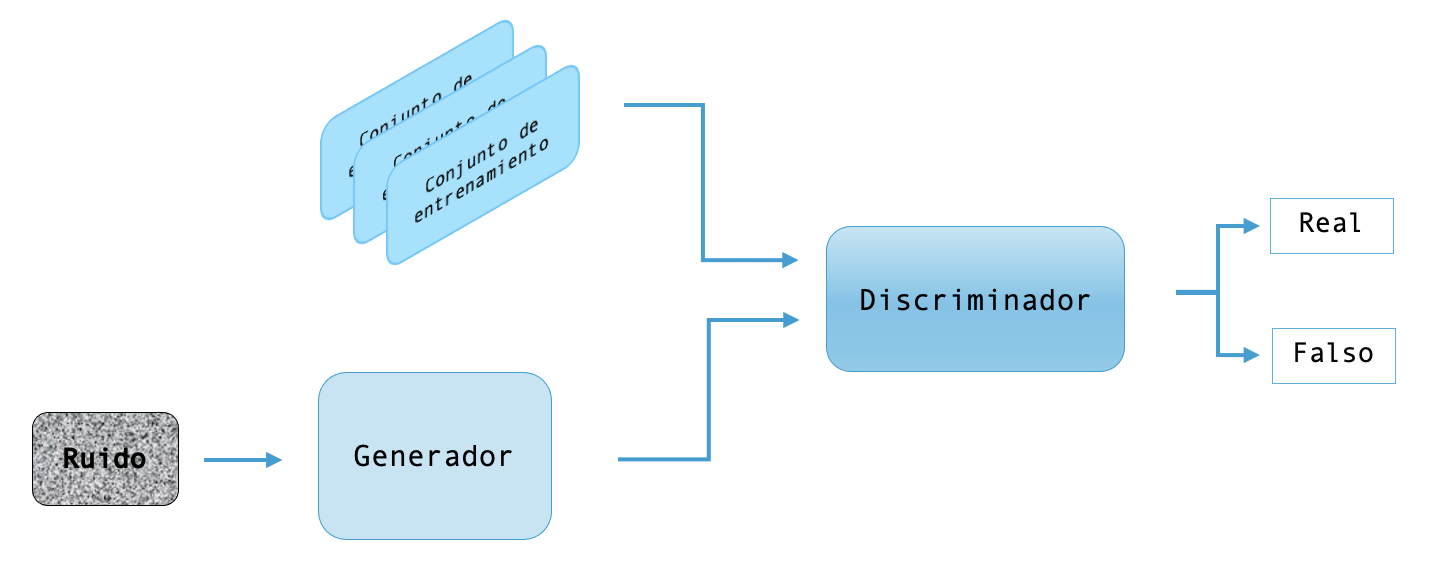
\includegraphics[width=0.9\textwidth]{entrenamiento}
    \caption{Proceso de entrenamiento de una GAN}
    \label{fig:entrenamiento-gan}
\end{figure}

\subsubsection{Efectos del ruido en la generación de imágenes}

En las Redes Generativas Adversarias, el ruido juega un papel crucial en el proceso de generación de imágenes, ya que sirve como entrada al generador para producir diversas representaciones a partir de una misma arquitectura. Dependiendo de la cantidad y la naturaleza del ruido inyectado, se pueden observar los siguientes efectos:
\begin{itemize}
    \item \textbf{Diversidad de las imágenes}:
    \begin{itemize}
        \item Ruido alto: Incluir un nivel elevado de ruido (alta desviación estándar) en el generador incrementa la variabilidad de las imágenes generadas. Esto puede resultar en una mayor diversidad de imágenes, aunque con el riesgo de introducir artefactos visuales o distorsiones no deseadas.
        \item Ruido bajo: Al reducir el nivel de ruido (baja desviación estándar), las imágenes tienden a ser más uniformes y menos diversas. Aunque esto puede reducir la aparición de artefactos, también limita la capacidad del modelo para generar imágenes novedosas.
    \end{itemize}
    
    \item \textbf{Calidad de la imagen}:
    \begin{itemize}
        \item Ruido alto: Un nivel elevado de ruido puede afectar negativamente la calidad de las imágenes generadas, haciéndolas borrosas o con artefactos visibles.
        \item Ruido bajo: Reducir el ruido puede mejorar la claridad de las imágenes, produciendo resultados más nítidos y definidos.
    \end{itemize}
    
    \item \textbf{Capacidad de generalización}:
    \begin{itemize}
        \item Ruido alto: Un generador entrenado con entradas de ruido alto tiende a generalizar mejor, ya que se entrena a partir de una amplia gama de entradas. Esto puede mejorar su rendimiento al generar imágenes realistas en distintos contextos.
        \item Ruido bajo: Al trabajar con menos variabilidad en las entradas, el generador puede ajustarse demasiado a los datos de entrenamiento, reduciendo su capacidad para generalizar y producir imágenes variadas en nuevos escenarios.
    \end{itemize}

    \item \textbf{Estabilidad del entrenamiento}:
    \begin{itemize}
        \item Ruido alto: Inyectar demasiado ruido puede hacer que el proceso de entrenamiento sea más inestable, dado que el modelo debe lidiar con una mayor variabilidad en las entradas. Esto puede provocar oscilaciones en la calidad de las imágenes generadas y dificultar la convergencia.
        \item Ruido bajo: Reducir el nivel de ruido tiende a estabilizar el entrenamiento, ya que las entradas son más consistentes. Sin embargo, esto puede limitar la capacidad del generador para mejorar en situaciones más complejas o variadas.
    \end{itemize}
\end{itemize}

En conclusión, la correcta gestión del nivel de ruido en las GANs es esencial para encontrar un equilibrio entre la diversidad de las imágenes generadas y la estabilidad del proceso de entrenamiento, lo que permite obtener imágenes de alta calidad y con buena capacidad de generalización.

\subsubsection{Aplicaciones}

Las Redes Generativas Adversarias han transformado diversos sectores gracias a su capacidad para generar datos y contenidos de alta calidad de manera artificial. Una de las aplicaciones más notables es la generación de imágenes realistas, donde pueden crear imágenes detalladas a partir de descripciones textuales o modificar imágenes existentes. Esto incluye tareas como la mejora de resolución de imágenes, la conversión de imágenes en blanco y negro a color, así como la creación de rostros, personajes y animales para industrias como la animación y los videojuegos.

Además, las GANs son fundamentales en la creación de datos sintéticos para el entrenamiento de modelos de aprendizaje automático. Generar datos sintéticos permite ampliar conjuntos de datos limitados o sesgados, mejorando el rendimiento de los modelos en tareas específicas. Por ejemplo, en el ámbito de la detección de fraudes pueden generar transacciones fraudulentas simuladas, permitiendo entrenar sistemas de detección de fraudes con una mayor precisión.

Otra aplicación clave es el completado de datos faltantes en conjuntos de datos incompletos. Las GANs pueden predecir y generar datos que llenen los vacíos en los conjuntos de datos, lo cual es especialmente útil en áreas como la cartografía geotérmica o la captura y almacenamiento de carbono. En estos casos pueden generar imágenes de la superficie subterránea a partir de datos topográficos limitados, proporcionando información crucial para la toma de decisiones en estos campos.

Estas aplicaciones representan solo una muestra de cómo las Redes Generativas Adversarias están impulsando avances significativos en distintas áreas, ampliando las fronteras de lo que es posible lograr mediante la inteligencia artificial y el aprendizaje profundo. Cada nueva implementación desafía los límites actuales, creando nuevas oportunidades para la innovación y el desarrollo tecnológico. \cite{aws-gan}


\subsection{Redes Generativas Adversarias Condicionales (cGAN)}
Las Redes Generativas Adversarias Condicionales (cGAN) son una extensión de las GAN convencionales, introducidas en 2014 por Mehdi Mirza y Simon Osindero \cite{datascientest-cgan}. A diferencia de las GAN estándar, que generan imágenes basadas únicamente en ruido aleatorio, las cGAN incorporan información adicional en forma de etiquetas condicionales, lo que permite un control más específico sobre las imágenes generadas. Esta capacidad de generar imágenes condicionales hace que las cGAN sean especialmente útiles en tareas que requieren resultados personalizados o categorizados según criterios específicos.

\subsubsection{Función de las Etiquetas}

Las etiquetas desempeñan un papel central en las cGAN, al proporcionar información contextual durante el proceso de entrenamiento. Estas etiquetas, que pueden representar categorías, atributos u otras características, se incorporan tanto en el generador como en el discriminador, permitiendo que ambos aprendan de forma más dirigida y precisa. Las funciones principales de las etiquetas en cada componente de la red son las siguientes:

\begin{itemize} 
    \item \textbf{Condición en el Generador:} Las etiquetas se concatenan con el vector de ruido que sirve como entrada al generador. Esta combinación de ruido y etiquetas actúa como una guía explícita, especificando el tipo de imagen que el generador debe crear. Por ejemplo, si la etiqueta corresponde a una categoría como ``gato'' o ``perro'', el generador utilizará esta información para generar una imagen que se ajuste a dicha categoría.
    \item \textbf{Condición en el Discriminador:} En el discriminador, las etiquetas se incorporan junto con las imágenes, permitiendo que el discriminador no solo evalúe si una imagen es real o generada, sino también si esa imagen corresponde a la etiqueta condicional proporcionada. Este proceso condiciona las decisiones del discriminador, mejorando su capacidad para detectar inconsistencias entre las imágenes generadas y las etiquetas asociadas.
\end{itemize}

Al integrar las etiquetas en ambos componentes, las cGAN permiten un nivel de control más fino sobre las imágenes generadas, lo que las convierte en una herramienta valiosa para aplicaciones donde se requiere una generación de imágenes personalizada o controlada. Esta capacidad condicional no solo mejora la flexibilidad de las GAN, sino que también amplía su aplicabilidad en campos como la creación de contenido visual, reconstrucción de imágenes y modelado tridimensional.

\subsubsection{Proceso de entrenamiento}
El proceso de entrenamiento de las cGAN sigue un enfoque similar al de las GAN convencionales, pero con la adición de información condicional en forma de etiquetas.

\begin{enumerate}
    \item \textbf{Inicialización}: Tanto el generador como el discriminador se inicializan en un estado de latencia preparados para el aprendizaje, al igual que en las GANs convencionales.
    
    \item \textbf{Generación y evaluación condicionada}: El generador toma una entrada de ruido aleatorio y las etiquetas condicionantes para generar datos falsos que se asemejen a los datos de entrenamiento reales. Estos datos generados son evaluados por el discriminador, que considera tanto la autenticidad de los datos como las etiquetas condicionantes.
    
    \item \textbf{Retroalimentación competitiva condicionada}: El discriminador proporciona retroalimentación al generador no solo sobre los errores en la generación de datos sino también sobre cómo se ajustan a las etiquetas condicionantes. Esto permite que el generador ajuste sus parámetros de manera más precisa.
    
    \item \textbf{Iteración condicionada}: El proceso de generación, evaluación y retroalimentación se repite en ciclos sucesivos, incorporando la información condicional en cada paso. Con cada ciclo de entrenamiento, tanto el generador como el discriminador mejoran su desempeño en relación con las etiquetas condicionantes, lo que resulta en una generación de datos más precisa y controlada.

\end{enumerate}

En resumen, las cGAN añaden una capa adicional de complejidad y control al proceso de entrenamiento de las GAN, permitiendo una generación de imágenes más personalizada y dirigida mediante el uso de etiquetas condicionantes.

\begin{figure}[H]
    \centering
    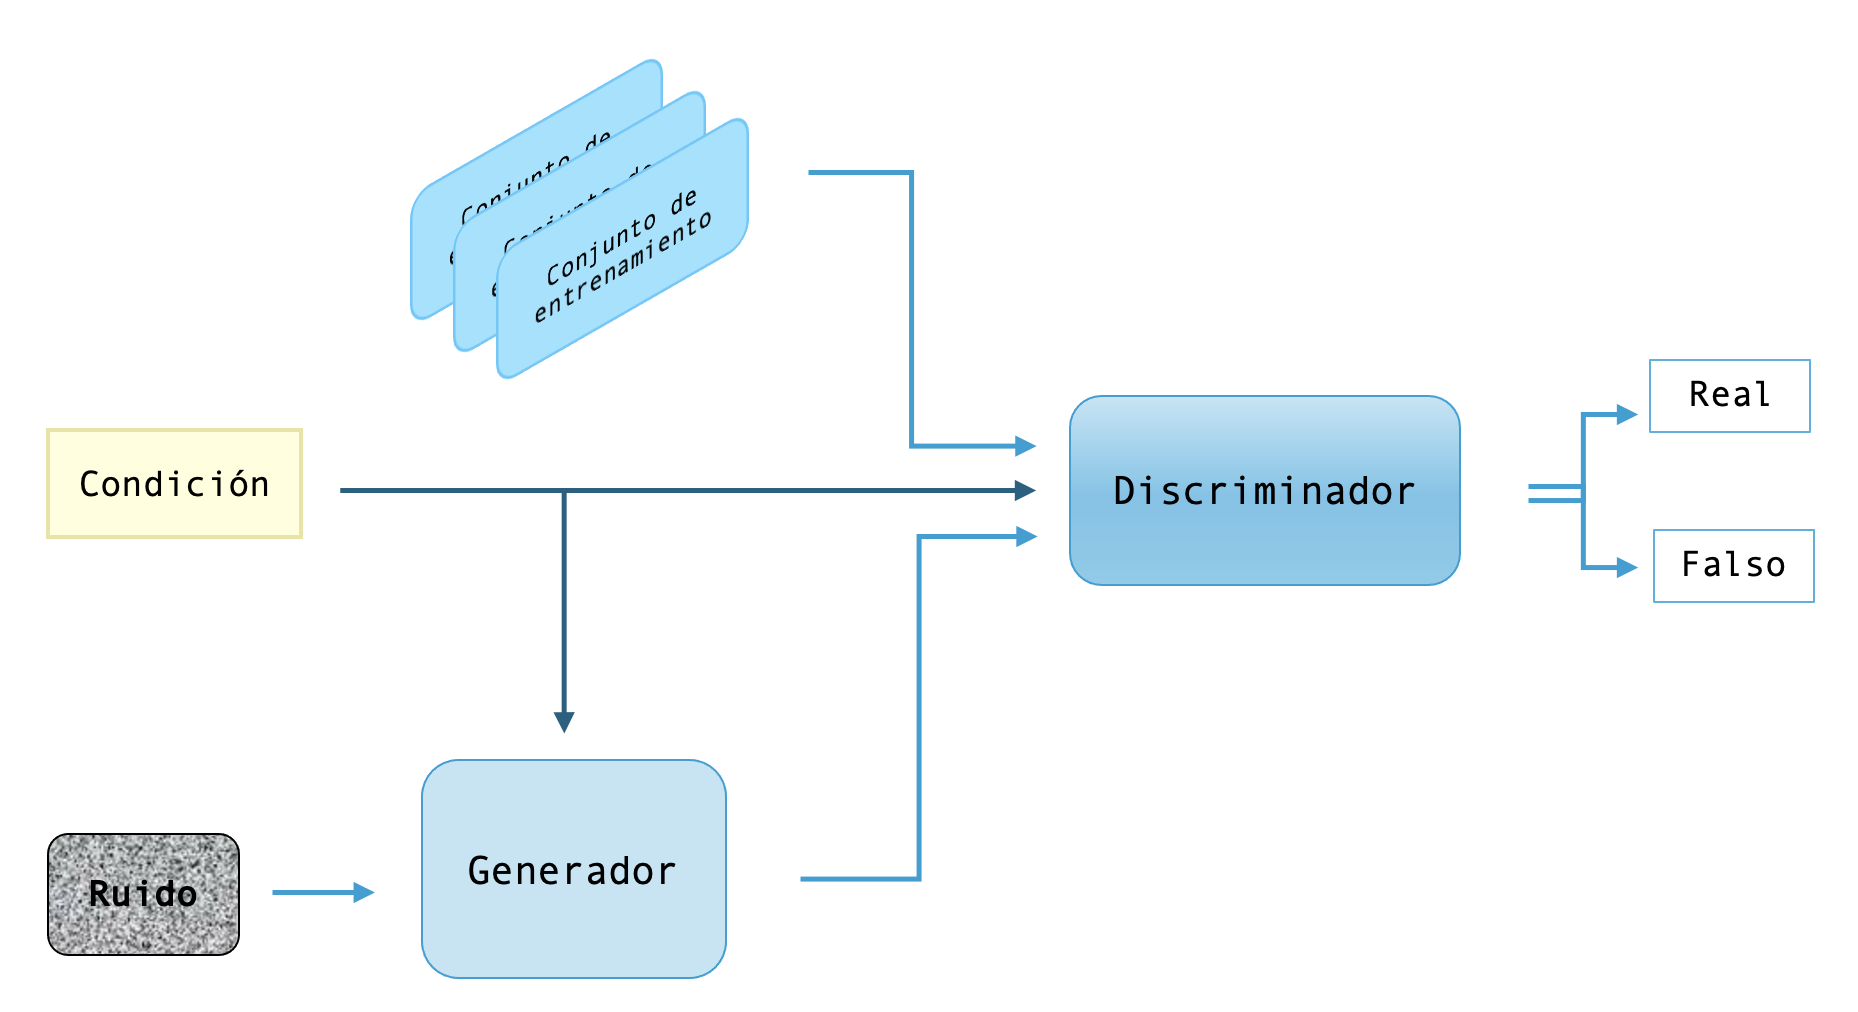
\includegraphics[width=0.9\textwidth]{entrenamiento-cgan}
    \caption{Proceso de entrenamiento de una cGAN}
    \label{fig:entrenamiento-cgan}
\end{figure}


\subsubsection{Aplicaciones}

Las cGAN han encontrado aplicaciones en una variedad de campos debido a su capacidad para generar imágenes de manera condicional. Algunas de las aplicaciones más destacadas incluyen:

\begin{itemize}
    \item \textbf{Traducción de Imagen a Imagen:} Las cGAN han revolucionado la traducción de imágenes con métodos como Pix2Pix, permitiendo la evolución de imágenes mediante la consideración de información adicional como etiquetas o mapas de bordes. Estas redes posibilitan la reconstrucción detallada de objetos a partir de bordes, la síntesis de fotografías de alta calidad guiadas por mapas de etiquetas, y la colorización precisa de imágenes en blanco y negro.
    
    \item \textbf{Creación de Imágenes a partir de Texto}: Es posible generar fotografías de alta calidad basadas en descripciones textuales. La riqueza del vocabulario utilizado permite la creación de imágenes sintéticas mucho más precisas y detalladas, capturando los matices y detalles específicos descritos en el texto.
    
    \item \textbf{Generación de Vídeo}: En el ámbito de la generación de vídeo, ofrecen la capacidad de predecir fotogramas futuros basados en una selección de imágenes previas. Esto es especialmente útil en aplicaciones como la interpolación de fotogramas y la generación de contenido de vídeo realista y fluido.
    
    \item \textbf{Generación de Rostros}: Estas redes pueden ser entrenadas para crear imágenes de rostros con características particulares, como el color del cabello, el color de los ojos y otros rasgos faciales, produciendo resultados realistas y detallados.
\end{itemize}

Esta flexibilidad y capacidad de adaptación hacen que las cGAN sean una herramienta poderosa en el campo del aprendizaje profundo y la generación de contenido visual.

\subsection{Redes Generativas Adversarias con Atención (AttnGAN)}
El modelo AttnGAN fue un gran avance en la generación de imágenes a partir de descripciones textuales . La característica clave de AttnGAN es su mecanismo de atención, que permite al modelo centrarse en diferentes partes de la descripción textual mientras genera la imagen. Este mecanismo de atención es particularmente útil para generar detalles complejos que se mencionan en las descripciones. \cite{xu2018attngan}

\subsubsection{Arquitectura}
La arquitectura de AttnGAN se compone de múltiples niveles de generación, cada uno enfocado en un nivel diferente de detalle en la imagen. La generación se lleva a cabo en tres niveles principales:

\begin{itemize}
    \item \textbf{Nivel de características globales}: El primer nivel se encarga de generar una versión básica de la imagen que capture la estructura global basada en la descripción textual. En este nivel, el generador utiliza un vector latente y el embedding de la frase para crear una representación inicial de la imagen.
    
    \item \textbf{Nivel de atención fina}: En el segundo nivel, el mecanismo de atención permite al generador centrarse en palabras específicas de la descripción para agregar detalles más finos a la imagen. Aquí, se utilizan representaciones de palabras para ajustar diferentes áreas de la imagen, como la textura o los colores.
    \item \textbf{Nivel de resolución alta}: Finalmente, el tercer nivel mejora aún más la resolución de la imagen y refina los detalles generados en los niveles anteriores, garantizando que la salida final tenga una alta calidad visual. Este proceso iterativo asegura que la imagen generada se mantenga coherente con la descripción textual proporcionada.
\end{itemize}

\subsubsection{DAMSM}
Un componente esencial de AttnGAN es el Deep Attentional Multimodal Similarity Model (DAMSM), diseñado para mejorar la coherencia entre las descripciones textuales y las imágenes generadas. DAMSM se entrena para alinear las representaciones de las descripciones de texto con las características de las imágenes, aprendiendo una representación conjunta de texto e imagen. Esto se logra mediante una pérdida de similitud que mide si una imagen generada se alinea con su descripción textual correctamente. El modelo intenta minimizar la distancia entre el embedding del texto y el embedding de la imagen correspondiente, ayudando al generador a producir imágenes que reflejen mejor las descripciones.

El DAMSM juega un papel crucial en el entrenamiento de AttnGAN, ya que no solo evalúa la calidad de la imagen generada, sino también cuán bien la imagen representa el contenido de la descripción. Este enfoque mejora significativamente la calidad semántica de las imágenes generadas, permitiendo que el modelo entienda descripciones más complejas y detalladas.

\subsubsection{Mecanismos de atención}
El concepto de atención se popularizó inicialmente en el campo del procesamiento de lenguaje natural (NLP) con el trabajo de Vaswani, titulado Attention is All You Need. Este enfoque demostró que, al permitir que un modelo se concentre en diferentes partes de una secuencia de entrada, se podían obtener mejores resultados en tareas como la traducción automática y el resumen de texto. \cite{vaswani2017attention}

La idea de la atención fue adaptada posteriormente para tareas de visión por computadora, como la generación de imágenes a partir de texto. En el caso de AttnGAN, el mecanismo de atención permite que el generador ajuste la contribución de cada palabra de la descripción en diferentes regiones de la imagen. Esto resulta en imágenes más precisas y detalladas en comparación con modelos que no utilizan atención.

\subsubsection{Métricas de evaluación}
Evaluar la calidad de las imágenes generadas por AttnGAN requiere el uso de métricas especializadas. Las dos métricas más comunes son el \textit{Inception Score} (IS) y la \textit{Fréchet Inception Distance} (FID):

\begin{itemize}
    \item \textbf{Inception Score (IS)}: Evalúa la calidad de las imágenes generadas analizando cómo una red preentrenada clasifica las imágenes. Un alto IS indica que las imágenes generadas son de alta calidad y que pertenecen a una variedad de categorías.
    
    \item \textbf{Fréchet Inception Distance (FID)}: Mide la distancia entre las distribuciones de características de las imágenes generadas y las imágenes reales. A diferencia del IS, la FID es más sensible a la calidad visual de las imágenes y es capaz de detectar artefactos en las imágenes generadas. Una FID más baja indica que las imágenes generadas son más similares a las imágenes reales.
\end{itemize}


\subsubsection{Proceso de entrenamiento}
El proceso de entrenamiento de AttnGAN sigue una estructura iterativa similar a las cGAN, pero incorpora un mecanismo de atención para mejorar la precisión en la generación de detalles visuales basados en descripciones textuales. El entrenamiento del modelo puede desglosarse en los siguientes pasos:
\begin{enumerate} 
    \item \textbf{Inicialización}: El generador y el discriminador se inicializan para el entrenamiento. Adicionalmente, el modelo DAMSM se entrena para alinear las representaciones textuales y visuales.
    \item \textbf{Generación basada en niveles de atención}: A partir de una descripción textual, el generador crea una representación inicial de la imagen que captura las características globales. Luego, mediante el mecanismo de atención, el modelo ajusta detalles específicos de acuerdo con palabras clave en la descripción.
    \item \textbf{Evaluación por el discriminador y DAMSM}: El discriminador evalúa la autenticidad de la imagen generada, mientras que DAMSM mide la similitud entre la descripción textual y la imagen producida. La combinación de estos dos enfoques permite ajustar el generador para mejorar tanto la autenticidad visual como la coherencia semántica.
    \item \textbf{Retroalimentación iterativa}: El proceso de generación y evaluación se repite en varias iteraciones. Cada ciclo ajusta los parámetros del generador para refinar la calidad de las imágenes, incorporando una correspondencia más precisa con las descripciones textuales.
\end{enumerate}

\subsubsection{Aplicaciones}
Al igual que las cGAN, AttnGAN ha encontrado aplicaciones en diversos campos que requieren una correspondencia precisa entre texto e imagen. Algunas de las aplicaciones más notables incluyen:
\begin{itemize} 
    \item \textbf{Creación de Imágenes a partir de Texto en Detalle}: AttnGAN es particularmente adecuado para generar imágenes con detalles complejos. Esto permite crear imágenes de calidad a partir de descripciones textuales detalladas, como se utiliza en diseño de moda, generación de paisajes o escenas específicas \cite{xu2018attngan}.
    \item \textbf{Edición de Imágenes Guiada por Texto}: AttnGAN permite la edición de imágenes existente utilizando descripciones textuales. Al cambiar palabras clave en el texto, el modelo puede modificar detalles específicos en la imagen sin alterar su estructura general.
    \item \textbf{Creación de Imágenes Médicas Sintéticas}: En el ámbito de la medicina, AttnGAN puede ser empleado para generar imágenes médicas sintéticas, especialmente en tareas que requieren la adición de características específicas en imágenes como tumores o lesiones en escaneos médicos, permitiendo una generación controlada en base a descripciones anatómicas \cite{liu2019medgan}.
    \item \textbf{Aplicaciones en Publicidad y Diseño Creativo}: AttnGAN es utilizado en la generación de contenido visual para campañas publicitarias, donde la descripción textual es crucial para representar productos con características específicas o crear ambientes temáticos detallados.
\end{itemize}

Con su capacidad de captar detalles finos y específicos a partir de descripciones textuales, AttnGAN representa una herramienta poderosa para aplicaciones que requieren precisión visual y semántica en la generación de imágenes.


\subsection{Procesamiento del lenguaje natural}
El procesamiento del lenguaje natural (NLP) es una disciplina de la inteligencia artificial que se encarga de dotar a los sistemas informáticos de la capacidad de comprender, interpretar, y generar lenguaje humano de manera eficiente. Utilizando una combinación de lingüística computacional y modelos de aprendizaje automático, el NLP permite a las máquinas procesar tanto texto como voz, con el fin de captar la intención y el sentimiento detrás de las comunicaciones humanas.

\begin{figure}[H]
    \centering
    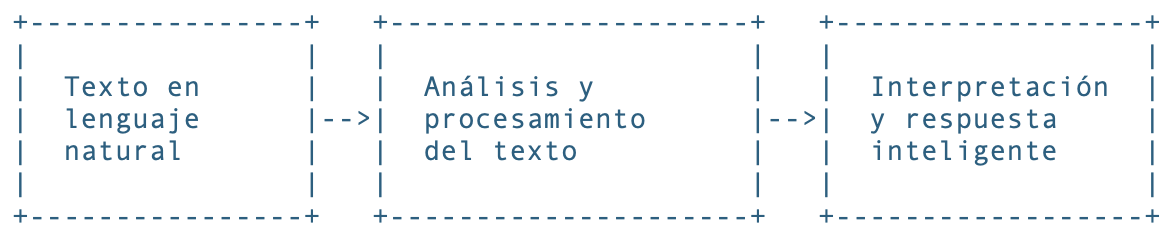
\includegraphics[width=0.8\textwidth]{lenguaje}
    \caption{Procesamiento del lenguaje}
    \label{fig:lenguaje}
\end{figure}

\subsubsection{Preparación del texto}
En esta etapa, se lleva a cabo la preparación del texto para su análisis posterior. Esto implica una serie de pasos de limpieza de datos, como la eliminación de caracteres especiales, la conversión a minúsculas y la exclusión de palabras vacías (stop words). El objetivo es asegurar que el texto esté en un formato adecuado para su procesamiento posterior.

\subsubsection{Tokenización}
Durante la tokenización, el texto se divide en unidades más pequeñas y significativas, conocidas como ``tokens''. Estos tokens pueden ser palabras individuales o frases completas, dependiendo del contexto y los objetivos del análisis. La tokenización proporciona una base fundamental para el procesamiento y análisis subsiguientes del texto, ya que permite a los algoritmos obtener una comprensión básica de la estructura y el contexto del texto.

En el caso de la tokenización de palabras, el texto se separa en tokens individuales basados en espacios en blanco, lo que permite identificar y aislar cada palabra dentro del texto. Por otro lado, en la tokenización de frases, el texto se divide en tokens basados en puntos o signos de puntuación, lo que facilita la identificación de unidades más grandes de texto con significado coherente.

\subsubsection{Representación del texto}
Adicionalmente, cada token generado durante el proceso de tokenización se convierte en una representación numérica comprensible por el modelo de procesamiento del lenguaje natural. Esto es esencial para permitir que el modelo comprenda y procese el texto de manera efectiva. Esta conversión se lleva a cabo mediante diversas técnicas de vectorización de texto, entre las cuales destacan la codificación one-hot y la incrustación de palabras (word embeddings).

\begin{itemize}
    \item La \textbf{codificación one-hot} consiste en asignar un valor binario único a cada token, creando un vector donde cada posición corresponde a una palabra única en el vocabulario. Por ejemplo, si tenemos un vocabulario de 1000 palabras, cada token se representaría como un vector de 1000 elementos, con un 1 en la posición que corresponde a la palabra en cuestión y ceros en todas las demás posiciones.
    \item Por otro lado, las \textbf{incrustaciones de palabras} (word embeddings) son representaciones vectoriales de palabras que capturan el significado semántico y la relación contextual entre ellas. Estas incrustaciones se generan mediante técnicas de aprendizaje automático y aprendizaje profundo, donde las palabras se representan como vectores densos de valores reales en un espacio de características de alta dimensionalidad.
\end{itemize}

Independientemente de la técnica utilizada, esta representación numérica de los tokens es esencial para alimentar el modelo de generación de imágenes en la siguiente etapa del proceso. Al transformar el texto en vectores numéricos, el modelo puede procesar la información de manera eficiente y generar contenido visual coherente y significativo basado en el contexto del texto de entrada.

\subsection{Generación de imágenes a partir de texto}
En la actualidad, se está presenciando un notable auge en el desarrollo de la Inteligencia Artificial Generativa, una vertiente diseñada para generar datos sintéticos innovadores basados en patrones extraídos de conjuntos de datos.

Este paradigma no se limita exclusivamente al procesamiento de datos en formato texto, sino que, además, abarca la capacidad de manipular imágenes, vídeos y audio; dando lugar a una diversidad de aplicaciones prometedoras que están emergiendo en distintos ámbitos.

\subsubsection{Ejemplos}
Los avances en inteligencia artificial están revolucionando la forma en que se diseñan productos industriales. Por ejemplo, se ha desarrollado un modelo llamado IA Midjourney que sirve como una herramienta creativa para representar ideas de manera rápida y efectiva; este modelo es capaz de transformar instrucciones detalladas en texto en representaciones visuales realistas de una amplia gama de productos industriales, desde cascos de motocicleta hasta zapatillas personalizadas de marcas reconocidas como Nike. Además, se ha observado que combinar múltiples tareas en una sola sesión puede mejorar la capacidad del modelo para generar imágenes variadas. Esta práctica también permite analizar los resultados en función de la popularidad del producto y explorar la variabilidad en las soluciones propuestas al representar objetos existentes.  \cite{calabuig2023modelos}

\begin{figure}[H]
    \centering
    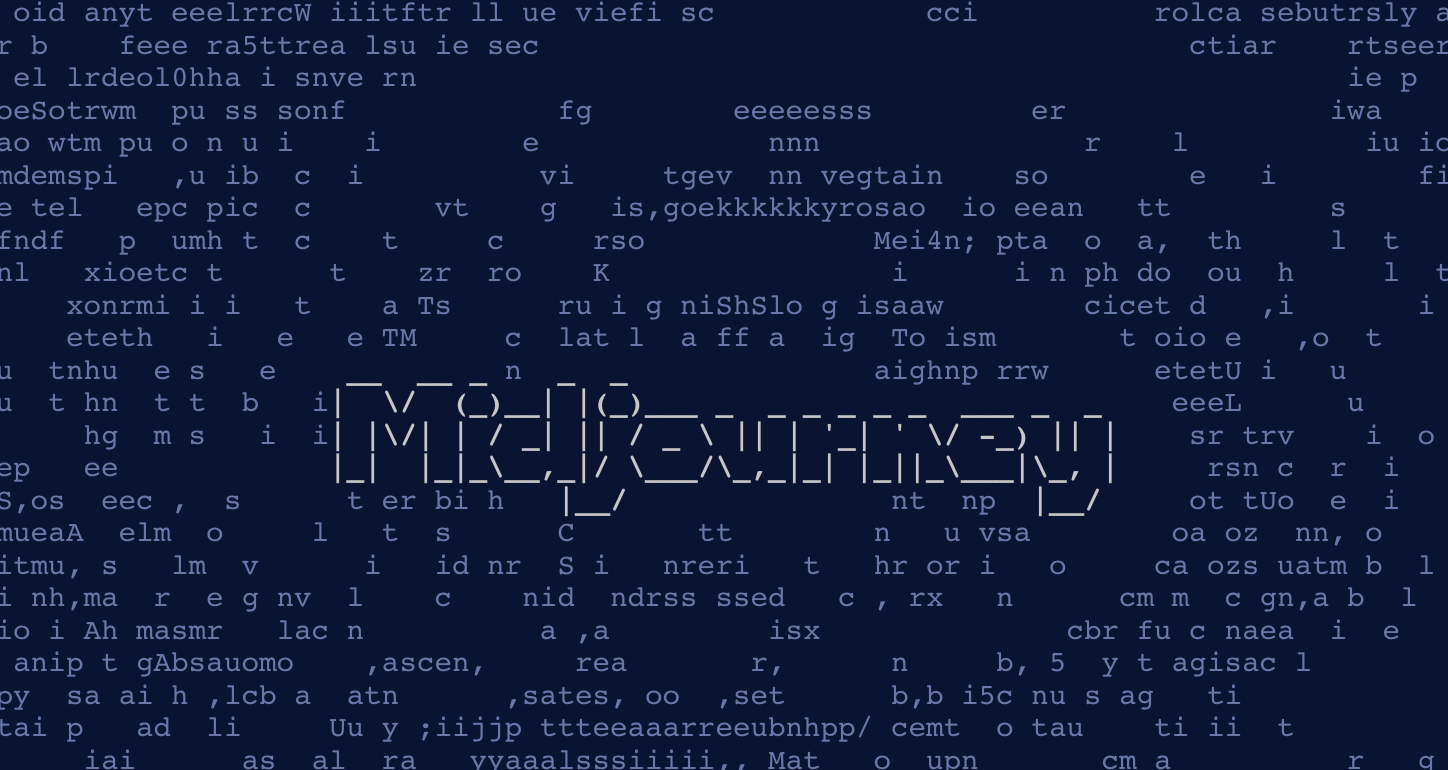
\includegraphics[width=0.6\textwidth]{midjourney}
    \caption{IA Midjourney}
    \label{fig:midjourney}
\end{figure}

\subsubsection{Consideraciones Éticas y de Privacidad}

El desarrollo de la Inteligencia Artificial Generativa (IAG) representa un cambio disruptivo en la forma de concebir, diseñar y producir contenidos digitales. Estas tecnologías permiten generar imágenes, vídeos, audios o incluso obras interactivas a partir de simples descripciones textuales, eliminando barreras técnicas y democratizando el acceso a herramientas de creación visual. El impacto de esta transformación ya se vislumbra en sectores como el diseño gráfico, la publicidad, la producción audiovisual, la educación y la realidad aumentada, entre otros.

No obstante, el avance acelerado de la IAG plantea una serie de dilemas éticos, sociales y legales de gran envergadura, que deben ser abordados de forma transversal y proactiva. A continuación, se detallan algunas de las principales consideraciones que afectan al uso responsable de estas tecnologías:

\begin{itemize}
    \item \textbf{Derechos de autor y propiedad intelectual:} Las obras generadas por algoritmos no cuentan con un creador humano directo, lo que plantea un vacío legal sobre su titularidad. ¿Pertenece el contenido al desarrollador del modelo, al usuario que lo genera, o a nadie? Esta indefinición complica tanto la comercialización como la protección de las creaciones, y puede incentivar prácticas poco éticas como la apropiación indebida o el plagio algorítmico.
    
    \item \textbf{Naturaleza jurídica de los contenidos generados:} Es necesario revisar las leyes de propiedad intelectual para incluir categorías específicas para las obras creadas mediante IAG. Además, surge la necesidad de establecer criterios para distinguir entre creaciones humanas, asistidas por IA y totalmente sintéticas.
    
    \item \textbf{Transparencia, trazabilidad y responsabilidad algorítmica:} En el contexto de la creación de contenido automatizado, es fundamental garantizar la trazabilidad del proceso generativo y la explicabilidad de los modelos. Esto es especialmente importante en aplicaciones sensibles (como medios de comunicación o salud), donde la veracidad, la intención y la autoría son factores críticos.
    
    \item \textbf{Identificación de contenidos sintéticos (deepfakes):} La creciente sofisticación de las imágenes y vídeos generados con IA plantea riesgos de desinformación, suplantación de identidad, manipulación política o fraudes digitales. La incorporación de marcas de agua digitales, metadatos incrustados o sistemas de verificación de autenticidad podría ser clave para distinguir entre contenido real y sintético.
    
    \item \textbf{Privacidad y uso de datos sensibles:} Los modelos de IA suelen entrenarse con grandes volúmenes de datos extraídos de internet o bases públicas. En muchos casos, estos datos incluyen rostros, ubicaciones, nombres o información privada que no ha sido recolectada con consentimiento explícito. Esto plantea serias implicaciones en términos de derechos fundamentales y cumplimiento normativo (como el RGPD en Europa).
    
    \item \textbf{Sesgos algorítmicos y reproducción de estereotipos:} Las IAG pueden reproducir o amplificar sesgos presentes en los datos con los que fueron entrenadas. Esto puede derivar en la generación de contenido discriminatorio o excluyente, reforzando estereotipos de género, raza o clase social. La revisión crítica del dataset y la introducción de mecanismos de mitigación de sesgos resultan imprescindibles.
    
    \item \textbf{Uso malintencionado o delictivo:} Como toda tecnología poderosa, la IAG puede ser empleada con fines maliciosos: generación de pornografía no consensuada, campañas de desinformación, fraude visual o creación de identidades falsas. Es necesario implementar barreras técnicas (filtros, restricciones de contenido, auditorías) y políticas públicas que regulen su uso y difusión.
    
    \item \textbf{Impacto en el empleo y la autoría creativa:} El auge de herramientas que automatizan procesos creativos podría afectar a profesionales del diseño, la ilustración o la escritura, especialmente en tareas de baja especialización. Es importante fomentar un marco de convivencia entre creatividad humana e inteligencia artificial, promoviendo la transparencia y el reconocimiento del trabajo original.
\end{itemize}

En resumen, el progreso de la Inteligencia Artificial Generativa ofrece un potencial inmenso, pero también una serie de riesgos éticos y legales que requieren atención urgente por parte de gobiernos, entidades tecnológicas, comunidades científicas y la ciudadanía en general. La implementación de principios como la transparencia, la equidad, la privacidad y la rendición de cuentas debe guiar el diseño y despliegue de estas tecnologías, para asegurar un desarrollo justo, inclusivo y sostenible.

\subsection{Modelos de Difusión y Stable Diffusion}

En los últimos años, los modelos generativos basados en procesos de difusión han cobrado una importancia creciente como alternativa a las arquitecturas GAN tradicionales. A diferencia de estas últimas, los modelos de difusión no requieren un discriminador y tienden a ser más estables durante el entrenamiento, además de ofrecer un mayor control semántico durante la generación.

\subsubsection{Fundamentos de los modelos de difusión}

Los modelos de difusión simulan un proceso estocástico en el que una imagen se convierte progresivamente en ruido gaussiano a través de una secuencia de pasos temporales. A continuación, el modelo se entrena para invertir este proceso, es decir, para reconstruir una imagen coherente a partir del ruido puro en varios pasos. Este enfoque fue formalizado inicialmente en los modelos DDPM (Denoising Diffusion Probabilistic Models) \cite{ho2020denoising}, y posteriormente optimizado en variantes como DDIM.

La formulación teórica se basa en procesos de difusión continua, descritos por la ecuación de Fokker–Planck:

\begin{equation}
\frac{\partial p(x,t)}{\partial t} = - \nabla \cdot (f(x)p(x,t)) + \nabla^2 (g(x)p(x,t))
\end{equation}

donde el objetivo es aprender una función de denoising $f_\theta(x,t)$ capaz de revertir el ruido inyectado en cada paso del proceso. La pérdida comúnmente empleada en estos modelos mide la diferencia entre el ruido predicho y el ruido real aplicado.

\subsubsection{Transición hacia la difusión latente}

Uno de los principales retos de los modelos de difusión tradicionales es su alto coste computacional, ya que operan directamente sobre imágenes de alta resolución. Para abordar esta limitación, surgieron los modelos de difusión latente, que trasladan el proceso de generación a un espacio comprimido de menor dimensión, manteniendo la información semántica esencial.

\subsubsection{Stable Diffusion}

Entre los modelos de difusión latente, destaca \textbf{Stable Diffusion} \cite{rombach2022high}, desarrollado por Stability AI y basado en la arquitectura Latent Diffusion Model (LDM). Este modelo ha ganado gran popularidad por su capacidad de generar imágenes fotorrealistas de alta calidad condicionadas por descripciones textuales (prompts), manteniendo una eficiencia computacional razonable.

Una de las características más destacables de Stable Diffusion es su disponibilidad como software de código abierto. Esto ha facilitado su adopción masiva en comunidades académicas, creativas y profesionales, y ha contribuido de forma significativa a la democratización del acceso a modelos generativos de alta calidad.

Stable Diffusion está compuesto por tres bloques principales:

\begin{itemize}
    \item Un \textbf{autoencoder variacional} (VAE), que se encarga de transformar imágenes del espacio RGB (alta dimensión) a un espacio latente comprimido y semánticamente significativo. Esta representación latente conserva la información visual esencial y permite operar con mayor eficiencia computacional. Una vez generado el resultado en el espacio latente, el VAE también es responsable de decodificarlo de nuevo a imagen visible, asegurando que se mantenga la coherencia visual respecto al contenido original.

    \item Un \textbf{modelo de difusión U-Net}, que actúa directamente sobre la representación latente de las imágenes. Esta red convolucional profunda está entrenada para eliminar progresivamente el ruido introducido en el espacio latente, reconstruyendo paso a paso una imagen coherente. Su arquitectura simétrica con conexiones de salto permite capturar tanto información global como detalles locales, y puede ser condicionada por información externa, como texto, durante el proceso de denoising.

    \item Un \textbf{codificador textual}, basado en modelos como CLIP o T5, cuya función es convertir la descripción textual (\textit{prompt}) en un vector de características semánticas. Este vector se utiliza como guía condicional en el proceso de generación. Gracias a los mecanismos de atención cruzada implementados en la U-Net, las representaciones textuales influyen directamente en distintas regiones de la imagen, permitiendo un alto grado de control sobre los elementos visuales generados en función del texto.
\end{itemize}


El modelo introduce un mecanismo de atención cruzada (cross-attention) que asocia partes específicas del texto con regiones concretas de la imagen, permitiendo un control detallado sobre el contenido generado.


\begin{figure}[H]
    \centering
    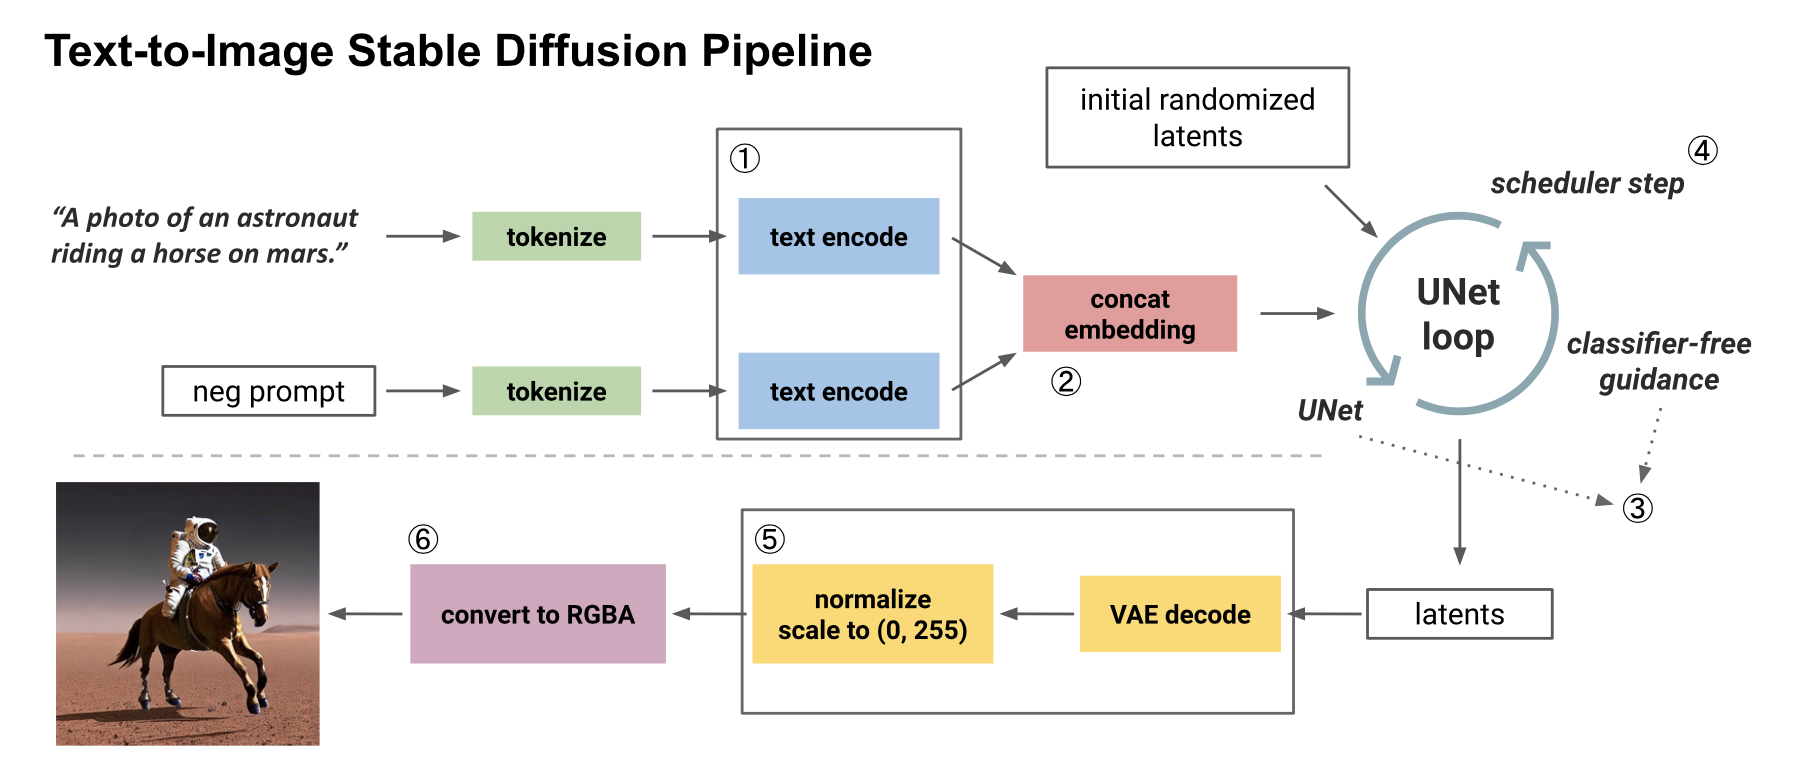
\includegraphics[width=0.9\textwidth]{stable_pipeline}
    \caption{Pipeline general del modelo Stable Diffusion. Fuente: \cite{mlc2023walkthrough}}
    \label{fig:sd_pipeline}
\end{figure}

\noindent La Figura \ref{fig:sd_pipeline} muestra el flujo de generación de imágenes en Stable Diffusion. A partir de un texto de entrada (\textit{prompt}), se obtiene un embedding que guía el proceso de denoising del modelo UNet en el espacio latente. Una vez finalizado el proceso, el resultado se decodifica a imagen mediante un VAE y se convierte a formato visual estándar.


\subsubsection{Ventajas frente a otras arquitecturas}

Stable Diffusion ofrece múltiples ventajas en comparación con arquitecturas anteriores como GANs o modelos híbridos como AttnGAN:

\begin{itemize}
    \item \textbf{Mayor coherencia semántica}: gracias al uso de embeddings textuales generados por modelos como CLIP o T5, y su integración mediante mecanismos de atención cruzada en la red U-Net, el modelo es capaz de asociar con precisión conceptos textuales con regiones específicas de la imagen generada. Esto resulta en una representación visual más fiel al contenido del prompt.

    \item \textbf{Mejor estabilidad}: a diferencia de las GAN, que dependen del equilibrio entre generador y discriminador, los modelos de difusión no requieren esta dinámica adversarial. Esto reduce significativamente problemas como el colapso de modo (donde el generador produce salidas repetitivas) o la inestabilidad del entrenamiento.

    \item \textbf{Coste computacional reducido}: al operar en un espacio latente comprimido mediante un autoencoder variacional, el modelo evita los altos requerimientos de memoria y procesamiento asociados con la manipulación directa de imágenes de alta resolución. Esta eficiencia permite su uso incluso en entornos con recursos limitados.

    \item \textbf{Modularidad}: la arquitectura de Stable Diffusion permite modificar, sustituir o mejorar individualmente componentes como el codificador de texto, el modelo de difusión o el decodificador VAE. Esto facilita la incorporación de mejoras incrementales sin tener que reentrenar todo el sistema desde cero.
\end{itemize}

Además, el trabajo de Rombach et al. \cite{rombach2022high} proporciona evidencia empírica de que el uso del espacio latente preserva la estructura semántica de las imágenes, manteniendo una alta calidad visual con menor coste computacional.

\subsubsection{Aplicaciones prácticas y uso en este trabajo}

El modelo Stable Diffusion ha demostrado ser eficaz en una amplia gama de aplicaciones prácticas:

\begin{itemize}
    \item \textbf{Generación de arte conceptual y prototipos visuales}: especialmente útil para diseñadores, artistas digitales y estudios creativos que buscan materializar ideas a partir de descripciones verbales.
    
    \item \textbf{Síntesis de datos para sistemas de visión artificial}: puede generar imágenes etiquetadas sintéticamente para entrenar clasificadores, detectores o segmentadores en entornos donde los datos reales son escasos o costosos de obtener.
    
    \item \textbf{Producción de contenido multimedia}: desde elementos gráficos en videojuegos hasta campañas publicitarias personalizadas, permite generar activos visuales adaptados a necesidades específicas.
\end{itemize}

En este proyecto, se ha utilizado Stable Diffusion como motor generativo dentro del sistema JMR. Gracias a una API REST, el usuario puede introducir un prompt textual en lenguaje natural y recibir una imagen generada que sirve como entrada visual al sistema CBIR (Content-Based Image Retrieval). Esta funcionalidad extiende las capacidades de búsqueda y análisis de la plataforma, haciendo el sistema más accesible y flexible.

\subsubsection{Limitaciones y desafíos actuales}

A pesar de sus beneficios, es importante considerar algunas limitaciones inherentes a Stable Diffusion:

\begin{itemize}
    \item \textbf{Velocidad de generación}: aunque más rápido que modelos de difusión que operan en pixel space, sigue siendo más lento que las GAN una vez entrenadas, ya que requiere múltiples pasos de inferencia para refinar la imagen.

    \item \textbf{Requisitos de memoria}: los modelos de difusión siguen siendo exigentes en términos de memoria GPU, especialmente al trabajar con prompts largos o al generar imágenes de alta resolución.

    \item \textbf{Falta de control preciso}: en casos donde el prompt es ambiguo, contradictorio o demasiado abierto, el modelo puede generar imágenes que no reflejan adecuadamente la intención del usuario.

    \item \textbf{Cuestiones éticas}: al estar entrenado con grandes volúmenes de datos de internet, el modelo puede reproducir sesgos sociales o generar contenido problemático. Además, existe un debate abierto sobre los derechos de autor en imágenes generadas a partir de entrenamiento con obras protegidas.
\end{itemize}

Estas limitaciones no invalidan su utilidad, pero deben ser cuidadosamente consideradas en contextos profesionales, educativos o institucionales donde la transparencia, la precisión y la responsabilidad son prioritarias. 

En consecuencia, cualquier despliegue real del sistema basado en Stable Diffusion debe ir acompañado de estrategias de mitigación ética, validación técnica rigurosa y un marco de uso responsable que garantice su fiabilidad y sostenibilidad a largo plazo.
